\documentclass[a4paper,12pt]{article}
\usepackage[T2A]{fontenc}
\usepackage[utf8]{inputenc}
\usepackage[english,russian]{babel}
\usepackage{listings}

\usepackage{amsmath}
\usepackage{MnSymbol}
\usepackage{wasysym}
\usepackage{indentfirst}

\usepackage{pgfplots}
\pgfplotsset{compat=1.9}

\usepackage{geometry}
\geometry{left=2cm}
\geometry{right=1.5cm}
\geometry{top=1cm}
\geometry{bottom=2cm}

\usepackage{graphicx}
\graphicspath{{img/}}
\DeclareGraphicsExtensions{.pdf,.png,.jpg}

\newcommand{\anonsection}[1]{\section*{#1}\addcontentsline{toc}{section}{#1}}

\lstset{
    language=C++,
    numbers=left,
    frame=single,
    texcl=true,
    basicstyle=\ttfamily
}

\begin{document}

\begin{titlepage}

    \begin{center}
        \large
        Государственное образовательное учреждение высшего профессионального образования\\
        “Московский государственный технический университет имени Н.Э.Баумана”
        \vspace{3cm}

        \textsc{Дисциплина: Анализ алгоритмов}
        \vspace{0.5cm}

        \textsc{Лабораторная работа №3}
        \vspace{3cm}

        {\LARGE ТРУДОЕМКОСТЬ СОРТИРОВОК}
        \vspace{3cm}

        Студент группы ИУ7-53,\\
        Степанов Александр Олегович
        \vfill
    \end{center}

    \begin{flushright}
        \begin{tabular}{l}
            Преподаватели:\\
            Строганов Юрий Владимирович\\
            Волкова Лилия Леонидовна
        \end{tabular}
    \end{flushright}

    \begin{center}

        2019 г.

    \end{center}

\end{titlepage}

\tableofcontents

\newpage
\anonsection{Введение}

В настоящее время необходимо сортировать большие объемы данных. Для этой
цели существуют алгоритмы сортировки, которые упорядочивают элементы в
списке.

Целями данной лабораторной работы является:

\begin{enumerate}
    \item Реализовать три различных алгоритма сортировки
    \item Теоретически вычислить эффективность алгоритмов
    \item Сравнить алгоритмы по времени и памяти
\end{enumerate}

\newpage
\section{Аналитическая часть}

Рассмотрим три сортировки:

\begin{itemize}
    \item Сортировка пузырьком
    \item Сортировка шейкером
    \item Быстрая сортировка
\end{itemize}

\subsection{Описание задачи}



\subsection{Пути решения}



\subsection{Выводы}

\newpage
\section{Конструкторская часть}

\subsection{IDEF0}

\begin{center}
    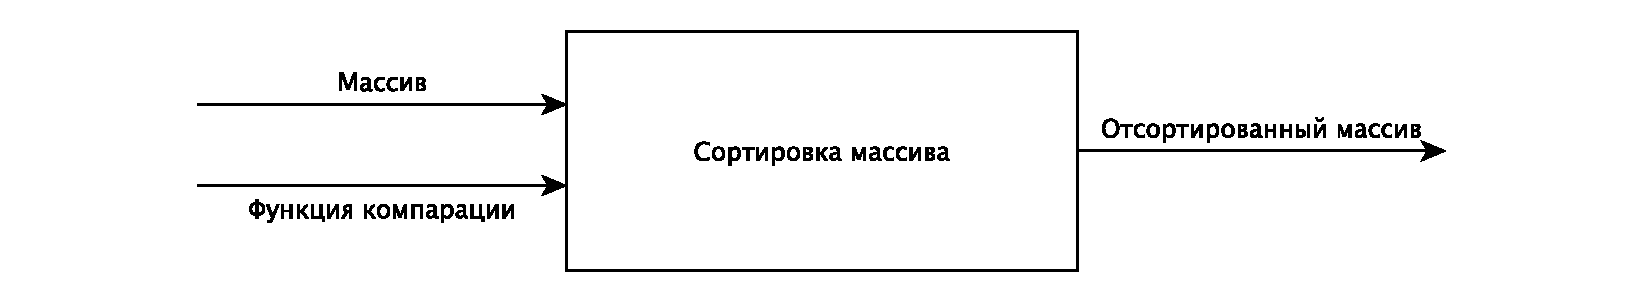
\includegraphics[scale=0.5]{IDEF0}
\end{center}

\subsection{Схемы алгоритмов}

\subsubsection{Сортировка пузырьком}

\begin{center}
    \includegraphics[scale=0.55]{Bubble}

    Схема 1. Сортировка пузырьком
\end{center}

\subsubsection{Сортировка шейкером}

\begin{center}
    \includegraphics[scale=0.97]{Shaker}

    Схема 2. Сортировка шейкером
\end{center}

\subsubsection{Быстрая сортировка}

\begin{center}
    \includegraphics[scale=0.45]{QSort}

    Схема 3. Быстрая сортировка
\end{center}

\subsection{Выводы}

\newpage
\section{Технологическая часть}

\subsection{Требования к программному обеспечению}

Программное обеспечение должно обеспечивать замер процессорного времени
выполнения каждого алгоритма. Проводятся замеры для случайно генерируемых
строк размерности до 1000. Выбранное ПО - MacOS.

\subsection{Средства реализации}

В качестве языка программирования был выбран C++. C++ компилируемый,
статически типизированный язык программирования общего назначения.
Данный язык имеет высокую скорость и богатую стандартную библиотеку,
содержащую необходимые контейнеры для данной работы, позволяющие
контролировать память благодаря объектно-ориентированному подходу
программирования.

\subsection{Листинг кода}

\begin{lstlisting}[caption=Сортировка пузырьком]
template < typename Type >
void BubbleSort< Type >::sort(std::vector< Type >& array,
                              bool (*comp)(Type, Type))
{
    for (int i = 0; i < array.size(); ++i) {
        for (int j = 0; j < array.size() - i - 1; ++j) {
            if (comp(array[j], array[j + 1])) {
                std::swap(array[j], array[j + 1]);
            }
        }
    }
}
\end{lstlisting}

\begin{lstlisting}[caption=Сортировка шейкером]
template < typename Type >
void ShakerSort< Type >::sort(std::vector< Type >& array,
                              bool (*comp)(Type, Type))
{
    int left = 0;
    int right = array.size() - 1;

    while (left <= right) {
        for (int i = left; i < right; ++i) {
            if (comp(array[i], array[i + 1])) {
                std::swap(array[i], array[i + 1]);
            }
        }
        --right;

        for (int i = right; i > left; --i) {
            if (comp(array[i - 1], array[i])) {
                std::swap(array[i - 1], array[i]);
            }
        }
        ++left;
    }
}
\end{lstlisting}

\begin{lstlisting}[caption=Быстрая сортировка]
template < typename Type >
void QSort< Type >::recursive(std::vector< Type >& array,
                              int start, int finish,
                              bool (*comp)(Type, Type))
{
    if (start < finish) {
        int left = start, right = finish;
        Type middle = array[(left + right) >> 1];

         while (left <= right) {
            while (comp(middle, array[left])) left++;
            while (comp(array[right], middle)) right--;

            if (left <= right) {
                std::swap(array[left], array[right]);
                ++left;
                --right;
            }
        }

        if (start < right) recursive(array, start, right, comp);
        if (left < finish) recursive(array, left, finish, comp);
    }
}
\end{lstlisting}

\subsection{Тестирование}

Для тестирования программы были заготовлены следующие тесты

\subsection{Выводы}

Для сравнения были реализованы 3 алгоритма на выбранном языке
программирования C++. Чтобы проверить правильность работы алгоритмов
были подготовлены тесты.

\newpage
\section{Экспериментальная часть}

\subsection{Примеры работ}

\subsection{Результаты тестирования}

\subsection{Замеры времени}

\begin{tikzpicture}
    \begin{axis}[
        title = Отсортированный массив,
        legend pos = north west,
        xlabel=Размер массива,
        ylabel=Милисекунды,
        grid = major,
        width = 0.8\paperwidth,
        height = 0.38\paperheight,
        line width = 1
    ]
        \legend{
            Сортировка пузырьком,
            Сортировка шейкером,
            Быстрая сортировка
        };
        \addplot[black] coordinates {
            (100, 54)
            (200, 480)
            (300, 990)
            (400, 1931)
            (500, 3256)
            (600, 5198)
            (700, 7921)
            (800, 11294)
            (900, 15785)
            (1000, 21199)
            (1100, 27480)
            (1200, 35323)
            (1300, 44344)
            (1400, 54314)
            (1500, 66169)
            (1600, 79273)
            (1700, 94383)
            (1800, 111104)
            (1900, 130147)
            (2000, 151057)
            (2100, 174071)
            (2200, 199279)
            (2300, 226997)
            (2400, 256903)
            (2500, 289446)
            (2600, 324843)
            (2700, 362309)
            (2800, 402484)
            (2900, 445472)
            (3000, 491389)
            (3100, 543209)
            (3200, 595428)
            (3300, 651489)
            (3400, 710303)
            (3500, 772716)
            (3600, 838642)
            (3700, 908582)
            (3800, 982140)
            (3900, 1061740)
            (4000, 1143214)
            (4100, 1228776)
            (4200, 1318504)
            (4300, 1412610)
            (4400, 1510895)
            (4500, 1616530)
            (4600, 1724451)
            (4700, 1836661)
            (4800, 1953636)
            (4900, 2075992)
            (5000, 2205651)
            (5100, 2338098)
            (5200, 2475531)
            (5300, 2620596)
            (5400, 2769172)
            (5500, 2922693)
            (5600, 3082142)
            (5700, 3249057)
            (5800, 3420220)
            (5900, 3597278)
            (6000, 3782922)
            (6100, 3972604)
            (6200, 4183597)
            (6300, 4413195)
            (6400, 4622532)
            (6500, 4845889)
            (6600, 5067437)
            (6700, 5295290)
            (6800, 5532806)
            (6900, 5774709)
            (7000, 6025377)
            (7100, 6281631)
            (7200, 6546718)
            (7300, 6817305)
            (7400, 7099640)
            (7500, 7385160)
            (7600, 7680146)
            (7700, 7981127)
            (7800, 8292025)
            (7900, 8610959)
            (8000, 8935735)
            (8100, 9270524)
            (8200, 9612418)
            (8300, 9966500)
            (8400, 10325515)
            (8500, 10693856)
            (8600, 11071532)
            (8700, 11455318)
            (8800, 11851570)
            (8900, 12255031)
            (9000, 12667819)
            (9100, 13088573)
            (9200, 13519645)
            (9300, 13960276)
            (9400, 14412407)
            (9500, 14873914)
            (9600, 15343144)
            (9700, 15822843)
            (9800, 16312289)
            (9900, 16811542)
            (10000, 17320621)
        };

        \addplot[dashed] coordinates {
            (100, 9)
            (200, 49)
            (300, 181)
            (400, 374)
            (500, 576)
            (600, 865)
            (700, 1313)
            (800, 1908)
            (900, 2585)
            (1000, 3420)
            (1100, 4421)
            (1200, 5602)
            (1300, 7040)
            (1400, 8670)
            (1500, 10495)
            (1600, 12551)
            (1700, 14868)
            (1800, 17466)
            (1900, 20358)
            (2000, 23555)
            (2100, 27361)
            (2200, 31249)
            (2300, 35500)
            (2400, 40120)
            (2500, 45213)
            (2600, 50895)
            (2700, 56947)
            (2800, 63199)
            (2900, 69906)
            (3000, 77288)
            (3100, 84960)
            (3200, 93233)
            (3300, 102168)
            (3400, 111539)
            (3500, 121285)
            (3600, 131796)
            (3700, 142878)
            (3800, 154616)
            (3900, 166919)
            (4000, 180067)
            (4100, 193575)
            (4200, 207832)
            (4300, 222717)
            (4400, 238312)
            (4500, 254742)
            (4600, 271753)
            (4700, 289510)
            (4800, 308128)
            (4900, 327565)
            (5000, 347546)
            (5100, 368387)
            (5200, 390279)
            (5300, 412879)
            (5400, 438201)
            (5500, 462532)
            (5600, 487806)
            (5700, 513945)
            (5800, 541104)
            (5900, 568951)
            (6000, 598068)
            (6100, 627730)
            (6200, 658416)
            (6300, 689970)
            (6400, 722773)
            (6500, 756503)
            (6600, 791188)
            (6700, 826998)
            (6800, 863852)
            (6900, 901793)
            (7000, 940736)
            (7100, 982529)
            (7200, 1024116)
            (7300, 1066632)
            (7400, 1110255)
            (7500, 1155066)
            (7600, 1201130)
            (7700, 1248440)
            (7800, 1297094)
            (7900, 1346750)
            (8000, 1397693)
            (8100, 1449837)
            (8200, 1504670)
            (8300, 1561150)
            (8400, 1617896)
            (8500, 1675985)
            (8600, 1734970)
            (8700, 1795270)
            (8800, 1856869)
            (8900, 1919805)
            (9000, 1984115)
            (9100, 2050002)
            (9200, 2117228)
            (9300, 2189848)
            (9400, 2260570)
            (9500, 2332962)
            (9600, 2406769)
            (9700, 2482027)
            (9800, 2558904)
            (9900, 2637011)
            (10000, 2718026)
        };

        \addplot[dotted] coordinates {
            (100, 7)
            (200, 24)
            (300, 50)
            (400, 79)
            (500, 107)
            (600, 143)
            (700, 187)
            (800, 243)
            (900, 304)
            (1000, 366)
            (1100, 437)
            (1200, 519)
            (1300, 605)
            (1400, 700)
            (1500, 803)
            (1600, 923)
            (1700, 1052)
            (1800, 1186)
            (1900, 1323)
            (2000, 1460)
            (2100, 1615)
            (2200, 1781)
            (2300, 1954)
            (2400, 2140)
            (2500, 2331)
            (2600, 2528)
            (2700, 2751)
            (2800, 2990)
            (2900, 3214)
            (3000, 3445)
            (3100, 3685)
            (3200, 3945)
            (3300, 4236)
            (3400, 4501)
            (3500, 4777)
            (3600, 5098)
            (3700, 5380)
            (3800, 5659)
            (3900, 5958)
            (4000, 6272)
            (4100, 6578)
            (4200, 6898)
            (4300, 7227)
            (4400, 7573)
            (4500, 7921)
            (4600, 8279)
            (4700, 8667)
            (4800, 9044)
            (4900, 9432)
            (5000, 9827)
            (5100, 10272)
            (5200, 10714)
            (5300, 11140)
            (5400, 11602)
            (5500, 12049)
            (5600, 12500)
            (5700, 12960)
            (5800, 13437)
            (5900, 13923)
            (6000, 14433)
            (6100, 14958)
            (6200, 15511)
            (6300, 16032)
            (6400, 16556)
            (6500, 17087)
            (6600, 17620)
            (6700, 18155)
            (6800, 18698)
            (6900, 19248)
            (7000, 19810)
            (7100, 20409)
            (7200, 21007)
            (7300, 21592)
            (7400, 22179)
            (7500, 22771)
            (7600, 23384)
            (7700, 23989)
            (7800, 24647)
            (7900, 25325)
            (8000, 25970)
            (8100, 26615)
            (8200, 27263)
            (8300, 27923)
            (8400, 28598)
            (8500, 29286)
            (8600, 30005)
            (8700, 30749)
            (8800, 31498)
            (8900, 32232)
            (9000, 32973)
            (9100, 33720)
            (9200, 34531)
            (9300, 35345)
            (9400, 36137)
            (9500, 36930)
            (9600, 37729)
            (9700, 38542)
            (9800, 39362)
            (9900, 40234)
            (10000, 41100)
        };
    \end{axis}
\end{tikzpicture}

\begin{tikzpicture}
    \begin{axis}[
        title = Обратно отсортированный массив,
        legend pos = north west,
        xlabel=Размер массива,
        ylabel=Милисекунды,
        grid = major,
        width = 0.8\paperwidth,
        height = 0.38\paperheight,
        line width = 1
    ]
        \legend{
            Сортировка пузырьком,
            Сортировка шейкером,
            Быстрая сортировка
        };
        \addplot[black] coordinates {
            (100, 294)
            (200, 1034)
            (300, 2598)
            (400, 5441)
            (500, 8836)
            (600, 12565)
            (700, 17689)
            (800, 24383)
            (900, 32987)
            (1000, 43384)
            (1100, 56225)
            (1200, 71197)
            (1300, 88705)
            (1400, 109347)
            (1500, 132772)
            (1600, 159632)
            (1700, 189579)
            (1800, 223656)
            (1900, 261292)
            (2000, 302658)
            (2100, 347985)
            (2200, 397609)
            (2300, 451855)
            (2400, 511226)
            (2500, 577318)
            (2600, 646997)
            (2700, 721577)
            (2800, 802066)
            (2900, 888437)
            (3000, 980839)
            (3100, 1081359)
            (3200, 1186146)
            (3300, 1297625)
            (3400, 1419408)
            (3500, 1546821)
            (3600, 1679880)
            (3700, 1820646)
            (3800, 1968625)
            (3900, 2126071)
            (4000, 2290149)
            (4100, 2462474)
            (4200, 2645339)
            (4300, 2834756)
            (4400, 3033133)
            (4500, 3242461)
            (4600, 3459033)
            (4700, 3687294)
            (4800, 3923119)
            (4900, 4171085)
            (5000, 4427042)
            (5100, 4695848)
            (5200, 4972185)
            (5300, 5262199)
            (5400, 5560948)
            (5500, 5872846)
            (5600, 6193412)
            (5700, 6527323)
            (5800, 6873802)
            (5900, 7229362)
            (6000, 7602149)
            (6100, 7982120)
            (6200, 8376914)
            (6300, 8785180)
            (6400, 9205965)
            (6500, 9639263)
            (6600, 10084762)
            (6700, 10545746)
            (6800, 11020084)
            (6900, 11508841)
            (7000, 12011019)
            (7100, 12528644)
            (7200, 13062362)
            (7300, 13612004)
            (7400, 14173155)
            (7500, 14750530)
            (7600, 15342791)
            (7700, 15948211)
            (7800, 16571551)
            (7900, 17211645)
            (8000, 17865734)
            (8100, 18537512)
            (8200, 19227595)
            (8300, 19938421)
            (8400, 20665078)
            (8500, 21405122)
            (8600, 22164303)
            (8700, 22944409)
            (8800, 23738014)
            (8900, 24549931)
            (9000, 25380980)
            (9100, 26231473)
            (9200, 27099010)
            (9300, 27996309)
            (9400, 28915671)
            (9500, 29844272)
            (9600, 30792424)
            (9700, 31759418)
            (9800, 32745153)
            (9900, 33748815)
            (10000, 34775989)
        };

        \addplot[dashed] coordinates {
            (100, 43)
            (200, 194)
            (300, 413)
            (400, 722)
            (500, 1198)
            (600, 1847)
            (700, 2727)
            (800, 4166)
            (900, 5721)
            (1000, 7575)
            (1100, 9799)
            (1200, 12461)
            (1300, 15612)
            (1400, 19237)
            (1500, 23347)
            (1600, 28231)
            (1700, 33492)
            (1800, 39373)
            (1900, 45933)
            (2000, 53390)
            (2100, 63841)
            (2200, 72986)
            (2300, 82808)
            (2400, 93209)
            (2500, 104713)
            (2600, 117338)
            (2700, 130834)
            (2800, 145080)
            (2900, 160559)
            (3000, 177514)
            (3100, 194896)
            (3200, 213791)
            (3300, 234027)
            (3400, 255204)
            (3500, 277977)
            (3600, 301643)
            (3700, 327148)
            (3800, 353488)
            (3900, 381670)
            (4000, 410906)
            (4100, 441990)
            (4200, 474260)
            (4300, 507824)
            (4400, 543140)
            (4500, 580282)
            (4600, 620917)
            (4700, 660965)
            (4800, 702875)
            (4900, 746554)
            (5000, 792165)
            (5100, 839421)
            (5200, 888530)
            (5300, 939609)
            (5400, 992564)
            (5500, 1047448)
            (5600, 1104328)
            (5700, 1165775)
            (5800, 1227084)
            (5900, 1290200)
            (6000, 1355443)
            (6100, 1423071)
            (6200, 1492669)
            (6300, 1564742)
            (6400, 1638875)
            (6500, 1718310)
            (6600, 1797708)
            (6700, 1879624)
            (6800, 1963857)
            (6900, 2050722)
            (7000, 2140019)
            (7100, 2233170)
            (7200, 2327351)
            (7300, 2423888)
            (7400, 2523084)
            (7500, 2625019)
            (7600, 2731841)
            (7700, 2839539)
            (7800, 2949747)
            (7900, 3062942)
            (8000, 3178830)
            (8100, 3299889)
            (8200, 3421794)
            (8300, 3546412)
            (8400, 3674924)
            (8500, 3808825)
            (8600, 3943272)
            (8700, 4080771)
            (8800, 4221642)
            (8900, 4367403)
            (9000, 4514053)
            (9100, 4664020)
            (9200, 4817779)
            (9300, 4976830)
            (9400, 5136913)
            (9500, 5300465)
            (9600, 5469676)
            (9700, 5640507)
            (9800, 5815120)
            (9900, 5994998)
            (10000, 6176640)
        };

        \addplot[dotted] coordinates {
            (100, 8)
            (200, 34)
            (300, 64)
            (400, 92)
            (500, 128)
            (600, 171)
            (700, 225)
            (800, 284)
            (900, 349)
            (1000, 418)
            (1100, 500)
            (1200, 591)
            (1300, 690)
            (1400, 799)
            (1500, 915)
            (1600, 1039)
            (1700, 1169)
            (1800, 1305)
            (1900, 1449)
            (2000, 1599)
            (2100, 1760)
            (2200, 1934)
            (2300, 2113)
            (2400, 2304)
            (2500, 2499)
            (2600, 2709)
            (2700, 2933)
            (2800, 3160)
            (2900, 3395)
            (3000, 3642)
            (3100, 3895)
            (3200, 4156)
            (3300, 4460)
            (3400, 4744)
            (3500, 5035)
            (3600, 5336)
            (3700, 5630)
            (3800, 5931)
            (3900, 6246)
            (4000, 6566)
            (4100, 6888)
            (4200, 7224)
            (4300, 7571)
            (4400, 7931)
            (4500, 8300)
            (4600, 8677)
            (4700, 9096)
            (4800, 9532)
            (4900, 9939)
            (5000, 10355)
            (5100, 10781)
            (5200, 11217)
            (5300, 11664)
            (5400, 12124)
            (5500, 12592)
            (5600, 13066)
            (5700, 13591)
            (5800, 14111)
            (5900, 14621)
            (6000, 15139)
            (6100, 15667)
            (6200, 16200)
            (6300, 16742)
            (6400, 17292)
            (6500, 17889)
            (6600, 18490)
            (6700, 19056)
            (6800, 19635)
            (6900, 20226)
            (7000, 20818)
            (7100, 21417)
            (7200, 22063)
            (7300, 22703)
            (7400, 23335)
            (7500, 23972)
            (7600, 24611)
            (7700, 25254)
            (7800, 25908)
            (7900, 26611)
            (8000, 27315)
            (8100, 27990)
            (8200, 28672)
            (8300, 29370)
            (8400, 30083)
            (8500, 30807)
            (8600, 31608)
            (8700, 32371)
            (8800, 33149)
            (8900, 33926)
            (9000, 34712)
            (9100, 35544)
            (9200, 36384)
            (9300, 37197)
            (9400, 38029)
            (9500, 38866)
            (9600, 39742)
            (9700, 41078)
            (9800, 42119)
            (9900, 42999)
            (10000, 43881)
        };
    \end{axis}
\end{tikzpicture}

\begin{tikzpicture}
    \begin{axis}[
        title = Случайный массив,
        legend pos = north west,
        xlabel=Размер массива,
        ylabel=Милисекунды,
        grid = major,
        width = 0.8\paperwidth,
        height = 0.38\paperheight,
        line width = 1
    ]
        \legend{
            Сортировка пузырьком,
            Сортировка шейкером,
            Быстрая сортировка
        };
        \addplot[black] coordinates {
            (100, 138)
            (200, 679)
            (300, 1529)
            (400, 3142)
            (500, 5719)
            (600, 9198)
            (700, 13884)
            (800, 20222)
            (900, 28231)
            (1000, 37961)
            (1100, 49971)
            (1200, 63792)
            (1300, 80378)
            (1400, 99973)
            (1500, 122056)
            (1600, 147411)
            (1700, 176063)
            (1800, 208635)
            (1900, 244096)
            (2000, 283437)
            (2100, 326796)
            (2200, 374390)
            (2300, 426398)
            (2400, 482930)
            (2500, 545840)
            (2600, 612076)
            (2700, 683490)
            (2800, 760661)
            (2900, 843132)
            (3000, 931241)
            (3100, 1025247)
            (3200, 1127314)
            (3300, 1234325)
            (3400, 1347835)
            (3500, 1468626)
            (3600, 1597476)
            (3700, 1731682)
            (3800, 1873207)
            (3900, 2022202)
            (4000, 2183165)
            (4100, 2347920)
            (4200, 2521003)
            (4300, 2704024)
            (4400, 2894229)
            (4500, 3093064)
            (4600, 3302669)
            (4700, 3519068)
            (4800, 3746644)
            (4900, 3981206)
            (5000, 4225382)
            (5100, 4481957)
            (5200, 4746525)
            (5300, 5022417)
            (5400, 5312562)
            (5500, 5607384)
            (5600, 5914215)
            (5700, 6232635)
            (5800, 6559918)
            (5900, 6900749)
            (6000, 7251487)
            (6100, 7615097)
            (6200, 7991972)
            (6300, 8381016)
            (6400, 8780538)
            (6500, 9195102)
            (6600, 9622059)
            (6700, 10062051)
            (6800, 10514617)
            (6900, 10980183)
            (7000, 11458893)
            (7100, 11952612)
            (7200, 12460636)
            (7300, 12982967)
            (7400, 13520351)
            (7500, 14071952)
            (7600, 14638640)
            (7700, 15222939)
            (7800, 15819089)
            (7900, 16432020)
            (8000, 17062305)
            (8100, 17707565)
            (8200, 18367118)
            (8300, 19041170)
            (8400, 19732035)
            (8500, 20442066)
            (8600, 21164461)
            (8700, 21905043)
            (8800, 22664317)
            (8900, 23441702)
            (9000, 24233931)
            (9100, 25046323)
            (9200, 25875207)
            (9300, 26724301)
            (9400, 27590374)
            (9500, 28475998)
            (9600, 29382997)
            (9700, 30304910)
            (9800, 31247399)
            (9900, 32212424)
            (10000, 33194225)
        };

        \addplot[dashed] coordinates {
            (100, 19)
            (200, 143)
            (300, 407)
            (400, 665)
            (500, 1058)
            (600, 1608)
            (700, 2451)
            (800, 3471)
            (900, 4757)
            (1000, 6323)
            (1100, 8191)
            (1200, 10367)
            (1300, 12923)
            (1400, 15878)
            (1500, 19262)
            (1600, 23126)
            (1700, 27721)
            (1800, 32572)
            (1900, 38031)
            (2000, 44081)
            (2100, 50882)
            (2200, 58321)
            (2300, 66275)
            (2400, 75294)
            (2500, 84822)
            (2600, 95098)
            (2700, 106353)
            (2800, 118487)
            (2900, 131572)
            (3000, 145506)
            (3100, 160410)
            (3200, 176349)
            (3300, 193051)
            (3400, 210811)
            (3500, 229823)
            (3600, 249949)
            (3700, 271053)
            (3800, 293462)
            (3900, 316905)
            (4000, 342022)
            (4100, 368020)
            (4200, 395619)
            (4300, 424085)
            (4400, 453997)
            (4500, 484805)
            (4600, 517015)
            (4700, 550901)
            (4800, 586026)
            (4900, 622514)
            (5000, 660396)
            (5100, 699728)
            (5200, 740666)
            (5300, 782987)
            (5400, 826666)
            (5500, 872207)
            (5600, 919401)
            (5700, 968249)
            (5800, 1020541)
            (5900, 1072852)
            (6000, 1127065)
            (6100, 1182858)
            (6200, 1240551)
            (6300, 1299873)
            (6400, 1361249)
            (6500, 1424615)
            (6600, 1490182)
            (6700, 1557534)
            (6800, 1626847)
            (6900, 1698331)
            (7000, 1771698)
            (7100, 1847662)
            (7200, 1925570)
            (7300, 2005621)
            (7400, 2089711)
            (7500, 2174017)
            (7600, 2260859)
            (7700, 2350078)
            (7800, 2441606)
            (7900, 2535490)
            (8000, 2631552)
            (8100, 2730238)
            (8200, 2831174)
            (8300, 2934615)
            (8400, 3040690)
            (8500, 3151012)
            (8600, 3262038)
            (8700, 3375875)
            (8800, 3492433)
            (8900, 3611676)
            (9000, 3733647)
            (9100, 3858196)
            (9200, 3985616)
            (9300, 4117659)
            (9400, 4250512)
            (9500, 4386037)
            (9600, 4524266)
            (9700, 4665371)
            (9800, 4809225)
            (9900, 4956418)
            (10000, 5106442)
        };

        \addplot[dotted] coordinates {
            (100, 12)
            (200, 47)
            (300, 93)
            (400, 153)
            (500, 260)
            (600, 416)
            (700, 583)
            (800, 809)
            (900, 1096)
            (1000, 1362)
            (1100, 1608)
            (1200, 1875)
            (1300, 2144)
            (1400, 2404)
            (1500, 2698)
            (1600, 2997)
            (1700, 3322)
            (1800, 3670)
            (1900, 4049)
            (2000, 4444)
            (2100, 4889)
            (2200, 5316)
            (2300, 5769)
            (2400, 6229)
            (2500, 6719)
            (2600, 7223)
            (2700, 7743)
            (2800, 8294)
            (2900, 8889)
            (3000, 9530)
            (3100, 10195)
            (3200, 10813)
            (3300, 11486)
            (3400, 12164)
            (3500, 12853)
            (3600, 13605)
            (3700, 14370)
            (3800, 15123)
            (3900, 15890)
            (4000, 16694)
            (4100, 17498)
            (4200, 18315)
            (4300, 19224)
            (4400, 20139)
            (4500, 21039)
            (4600, 21984)
            (4700, 22931)
            (4800, 23930)
            (4900, 24910)
            (5000, 25929)
            (5100, 26938)
            (5200, 27984)
            (5300, 29113)
            (5400, 30236)
            (5500, 31348)
            (5600, 32481)
            (5700, 33673)
            (5800, 34874)
            (5900, 36060)
            (6000, 37261)
            (6100, 38531)
            (6200, 39863)
            (6300, 41150)
            (6400, 42475)
            (6500, 43867)
            (6600, 45201)
            (6700, 46568)
            (6800, 48014)
            (6900, 49461)
            (7000, 50876)
            (7100, 52402)
            (7200, 53870)
            (7300, 55371)
            (7400, 56931)
            (7500, 58487)
            (7600, 60049)
            (7700, 61681)
            (7800, 63290)
            (7900, 64892)
            (8000, 66593)
            (8100, 68282)
            (8200, 69968)
            (8300, 71759)
            (8400, 73476)
            (8500, 75218)
            (8600, 77018)
            (8700, 78845)
            (8800, 80770)
            (8900, 82596)
            (9000, 84425)
            (9100, 86340)
            (9200, 88277)
            (9300, 90238)
            (9400, 92164)
            (9500, 94096)
            (9600, 96160)
            (9700, 98222)
            (9800, 100323)
            (9900, 102397)
            (10000, 104486)
        };
    \end{axis}
\end{tikzpicture}

\subsection{Выводы}


\newpage
\anonsection{Заключение}

\newpage
\anonsection{Список использованной литературы}
\end{document}
